\documentclass{spisok-article}

\usepackage{subcaption}

\newcommand{\prevGender}{78,87\%}
\newcommand{\prevAge}{3,69}

\newcommand{\bestGender}{82,46\%}
\newcommand{\bestAge}{3,38}

\title{Определение демографических характеристик пользователей
  сайта Last.fm на основе анализа их музыкальных интересов
}

\author{Семёнов А. С., магистрант кафедры КТ университета ИТМО,
  semkagtn@gmail.com
}

\begin{document}

\maketitle

\begin{abstract}
В данной работе представлено два подхода к определению пола и
возраста пользователей сайта Last.fm\footnote{http://www.last.fm}
на основе прослушиваемых ими музыкальных исполнителей.
Достигнутые результаты: точность определения пола~--- \bestGender,
средняя абсолютная ошибка определения возраста~--- \bestAge.
\end{abstract}


\section{Введение}

В наше время Интернет играет большую роль. Миллионы людей
по всему миру пользуются социальными сетями, интернет-магазинами
и другими онлайн-сервисами. Пользователи оставляют о себе
огромное количество информации в открытом доступе даже 
не замечая этого. Благодаря этому появляется возможность
определять <<скрытые>> характеристики пользователей на основе
имеющейся информации. Такими характеристиками, например, 
являются пол и возраст. Многие сайты предоставляют возможность 
указывать эти параметры, но часто это не является обязательным
требованием. Отсюда возникает задача устранения неполноты в 
данных. Восстановление недостающих характеристик пользователей 
позволяет улучшить различные системы
рекомендаций~\cite{recommender2001,recommender2005}.

Существует множество исследований, показывающих возможность 
определять пол и возраст на основе косвенных признаков.
В работе~\cite{burger2006} исследовалась зависимость 
между текстом блогеров и их возрастом.
Авторы работ~\cite{peersman2011,turdakov2013,schwartz2013} 
предлагают подходы к определению демографических характеристик 
на основе сообщений пользователей. Текст~--- не единственная
информация, которая может быть использована. Например, в
работе~\cite{rosenthal2011} учитывалось также
поведение пользователей. А в работе~\cite{farseev2015}
для определения демографических характеристик использовались
также фотографии и геолокация пользователей.

Использование информации о музыке, которую слушают пользователи, 
также возможно. В статье~\cite{christenson1988} была показана
корреляция между предпочтением определённых жанров и полом у
группы студентов. В работе~\cite{liu2012} пол и возраст определялся
по истории прослушиваний музыкальных композиций.
В исследовании~\cite{wu2014} используется 50 наиболее
прослушиваемых композиций каждого пользователя сайта Last.fm.

В рамках настоящей работы предложены подходы к определению
демографических характеристик пользователей на данных, которые
использовались в последней упомянутой статье. Предполагается,
что описанные методы могут помочь улучшить существующие алгоритмы,
не использующие информацию о музыке пользователей.

Задача определения пола решалась как задача 
классификации, а задача определения возраста~--- как
задача восстановления регрессии.


\section{Описание набора данных}

Набор данных содержит $96807$ пользователей.
Каждый пользователь описан 50 исполнителями из списка наиболее
прослушиваемых им музыкальных композиций. Эти данные были получены
с сайта Last.fm при помощи метода API 
\textit{User.getTopTracks}\footnote{
http://www.last.fm/api/show/user.getTopTracks}, который возвращает
самые прослушиваемые музыкальные композиции заданного пользователя.
Музыкальные композиции отсортированы в порядке убывания по числу
прослушиваний. Из этого списка были извлечены исполнители (с сохранением
порядка). Таким образом, исполнители, описывающие
пользователя, могут повторяться.
У каждого пользователя указан пол и число полных лет.

Следует отметить некоторые особенности выборки. Во-первых,
мужчин в ней содержится больше, чем женщин (см. Рис.~\ref{fig:gender}).
Во-вторых, возраст пользователь сильно смещён в сторону молодого
поколения (см. Рис.~\ref{fig:age}).

\begin{figure}[h!]
\centering
\begin{subfigure}[а]{0.42\textwidth}
    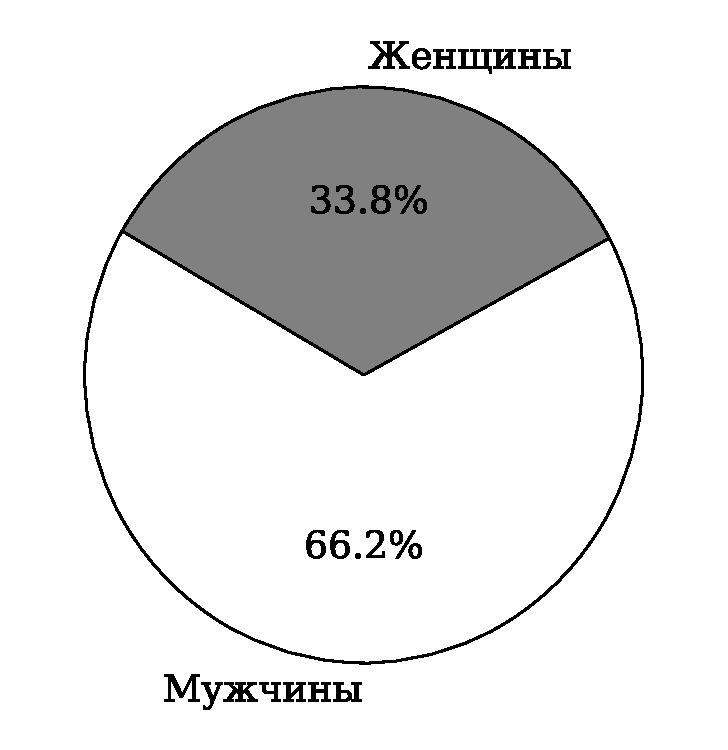
\includegraphics[width=\textwidth]{figures/gender-pie.pdf}
    \caption{Пол}
    \label{fig:gender}
\end{subfigure}
\begin{subfigure}[б]{0.57\textwidth}
    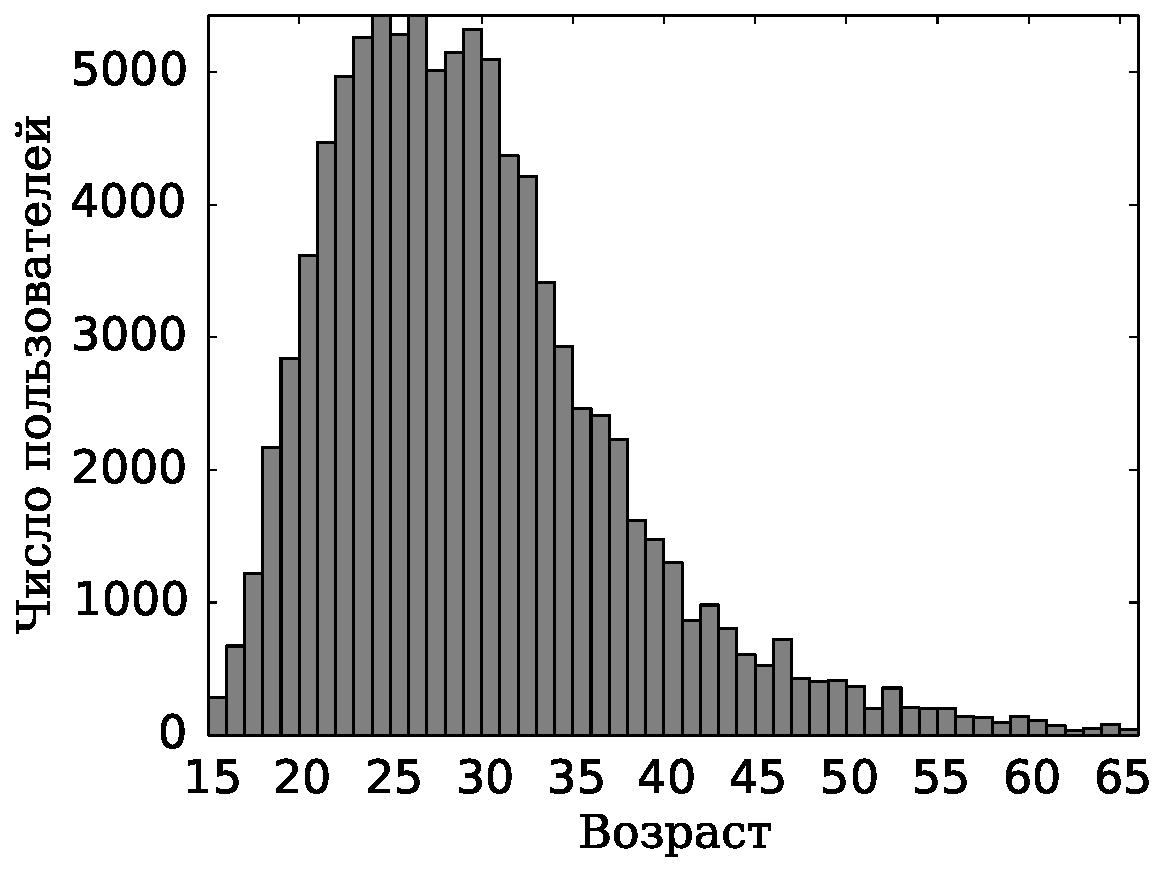
\includegraphics[width=\textwidth]{figures/age-histogram.pdf}
    \caption{Возраст}
    \label{fig:age}
\end{subfigure}
\caption{Распределение демографических характеристик в выборке}
\end{figure}

Выборка разбита на обучающую и контрольную ($48404$ и $48403$
пользователей соответственно) таким образом, чтобы распределение
полов в каждой выборке было одинаковым.

\section{Преобразование данных в векторное пространство}

В данном разделе описаны подходы, позволяющие преобразовать
пользователей в численные векторы, пригодные для
использования в качестве признакового описания для решения
задачи классификации или восстановления регрессии.

\subsection{Подход на основе матрицы термин--документ}
Пользователей можно рассматривать как <<документы>>, в
которых терминами являются исполнители. Отсюда на основе
подхода "bag of words"~\cite{manning} 
возникает матрица $D = \{d_{ij}\}$, где элемент $d_{ij}$
обозначает степень принадлежности термина $i$ документу $j$.
В качестве функции степени принадлежности часто используется формула TF-IDF:
\begin{equation} \label{eq:tfidf}
    d_{ij} = \mathrm{tf}_{ij} \cdot \log{\frac{n}{\mathrm{df}_{i}}},
\end{equation}
где $\mathrm{tf}_{ij}$~--- число встреч термина $i$ в документе $j$,
$\mathrm{df}_{i}$~--- число документов, в которых встречается термин $i$,
$n$~--- общее число документов.
Формула TF-IDF, может быть обобщена следующим образом:
\begin{equation} \label{eq:general_tfidf}
d_{ij} = 
\begin{cases}
    0,& \mathrm{tf}_{ij} = 0,\\
    l(\mathrm{tf}_{ij}) \cdot g(\frac{n}{\mathrm{df}_{i}}),& \mathrm{tf}_{ij} \ne 0,
\end{cases}
\end{equation}
где $l(x)$ и $g(x)$~--- неубывающие и неотрицательные функции.

Матрица термин--документ описывает каждый документ через вектор
терминов. Размерность векторов в нашей задаче оказывается
крайне большой~--- $96891$, что обуславливает необходимость 
применить метод снижения размерности. Ввиду сильной разреженности
матрицы для этой цели был выбран метод LSI~\cite{lsi}, основанный
на сингулярном разложении, а именно его реализация из библиотеки
gensim\footnote{https://radimrehurek.com/gensim/}. Произвольным
образом была выбрана размерность равная $200$. 

Таким образом, каждый пользователь описан $200$ числовыми признаками. 
Стоит отметить, что вектор каждого пользователя был 
нормализован таким образом, чтобы его длина была равной единице.

\subsection{Подход на основе модели Word2Vec}
Модель Word2Vec~\cite{word2vec} позволяет преобразовать словарь
терминов в численные векторы одинаковой размерности. Таким
образом, каждый документ можно представить в виде
последовательности численных векторов. Основываясь на
предположении о том, что чем выше исполнитель находится в
рейтинге пользователя, тем более <<значимым>> он является,
можно построить вектор, представляющий пользователя, следующим
образом:

\begin{equation} \label{eq:doc2vec}
    d_{i} = \sum_{n}{f(n) \cdot w_{in}},
\end{equation}
где $w_{in}$~--- термин (исполнитель), который находится
у пользователя $i$ на позиции с номером $n$; $f(n)$~---
невозрастающая неотрицательная функция на промежутке $[1; 50]$
(ввиду того, что каждый документ состоит 
не более чем из $50$ терминов).

Использовалась реализация модели Word2Vec из 
библиотеки \textit{gensim} с параметрами:
\textit{size} = $200$ и \textit{window} = $25$.

Таким образом, каждый пользователь описан численным вектором,
размерность которого равна $200$. Стоит отметить, что численные
векторы пользователей были преобразованы так, чтобы
каждая координата имела математическое ожидание равное нулю и
среднеквадратическое отклонение равное единице.


\section{Этап обучения и результаты}

Для решения задач классификации или регрессии использовался
метод опорных векторов (Support Vector Machine)~\cite{svm},
а именно его реализация
из библиотеки scikit-learn\footnote{http://scikit-learn.org}.
В качестве функции ядра использовалось ядро \textit{RBF}, а параметры
\textit{gamma} и \textit{C} настраивались на обучающей выборке
методом GridSearchCV, который реализован в упомянутой библиотеке.
Значения параметра \textit{C} были взяты из множества
$\{0{,}1; 0{,}5; 1; 3\}$, значения параметра \textit{gamma} из~--- 
$\{0{,}001; 0{,}01; 0{,}1; 1; 8; 16; 32; 64\}$. Выбор параметров
основан на рекомендации из статьи~\cite{svm2003recom}, где
авторы рекомендуют выбирать последовательности, которые растут нелинейно.

Качество классификатора или регрессора определялось на контрольной
выборке. Метрикой для задачи определения пола была выбрана точность,
а для задачи определения возраста~--- средняя абсолютная ошибка.

Результаты с использованием подхода на основе матрицы
термин--документ при различных функциях $l(x)$ и $g(x)$ из
уравнения~\ref{eq:general_tfidf} приведены в
таблице~\ref{tab:tfidf_results}.

\begin{table}[h!]
\centering
\begin{tabular}{|c|c|c|c|}
\hline
\thd{\boldmath$l(x)$} & \thd{\boldmath$g(x)$} & \thd{Определение пола} & \thd{Определение возраста} \tabularnewline
\hline
$1$ & $1$ & \textbf{82,46\%} & \textbf{3,54} \tabularnewline
\hline
$\log{x}$ & $1$ & 81,58\% & 3,64 \tabularnewline
\hline
$\log{x}$ & $\log{x}$ & 81,67\% & 3,57 \tabularnewline
\hline
$\log{x}$ & $\sqrt{x}$ & 80,04\% & 3,76 \tabularnewline
\hline
$\sqrt{x}$ & $1$ & 81,73\% & 3,63 \tabularnewline
\hline
$\sqrt{x}$ & $\log{x}$ & 81,76\% & 3,57 \tabularnewline
\hline
$\sqrt{x}$ & $\sqrt{x}$ & 79,78\% & 3,77 \tabularnewline
\hline
$x$ & $1$ & 79,45\% & 3,92 \tabularnewline
\hline
$x$ & $\log{x}$ & 79,67\% & 3,85 \tabularnewline
\hline
$x$ & $\sqrt{x}$ & 78,75\% & 3,88 \tabularnewline
\hline
\end{tabular}
\caption{Результаты с использованием подхода термин--документ}
\label{tab:tfidf_results}
\end{table}

Результаты с использованием подхода на основе модели
Word2Vec при различных функциях $f(n)$ из уравнения~\ref{eq:doc2vec}
приведены в таблице~\ref{tab:doc2vec_results}.

\begin{table}[h!]
\centering
\begin{tabular}{|c|c|c|}
\hline
\thd{\boldmath$f(n)$} & \thd{Опредление пола} & \thd{Определение возраста} \tabularnewline
\hline
$1$ & 78,12\% & 3,97 \tabularnewline
\hline
$\frac{1}{\log{n + 1}}$ & 79,61\% & 3,59 \tabularnewline
\hline
$\frac{1}{n^2}$ & 78,66\% & 4,02 \tabularnewline
\hline
$\frac{1}{n}$ & 80,22\% & 3,75 \tabularnewline
\hline
$\frac{1}{\sqrt{n}}$ & \textbf{81,46\%} & \textbf{3,38} \tabularnewline
\hline
$51 - n$ & 77,85\% & 4,03 \tabularnewline
\hline
$\log{51} - \log{n}$ & 78,16\% & 3,95 \tabularnewline
\hline
$\sqrt{51} - \sqrt{n}$ & 78,12\% & 3,98 \tabularnewline
\hline
\end{tabular}
\caption{Результаты с использованием подхода на основе модели Word2Vec}
\label{tab:doc2vec_results}
\end{table}

Сравнение лучших результатов, достигнутых в рамках настоящего
исследования, (\textit{best}) и полученных ранее в 
работе~\cite{wu2014} (\textit{baseline}) приведено в
таблице~\ref{tab:total_results}.

\begin{table}[h!]
\centering
\begin{tabular}{|c|c|c|}
\hline
\thd{Тип задачи} & \thd{best} & \thd{baseline} \tabularnewline
\hline
Определение пола & \textbf{\bestGender} & \prevGender \tabularnewline
\hline
Определение возраста & \textbf{\bestAge} & \prevAge \tabularnewline
\hline
\end{tabular}
\caption{Сравнение результатов с результатами, полученными ранее}
\label{tab:total_results}
\end{table}

Следует отметить, что размерность пространства признакового
описания была выбрана произвольно. Изменение этой величины
может сильно влиять на конечный результат. Изменение <<сетки>>
значений, по которой настраивались параметры метода опорных векторов,
также может сильно влиять на результат.

\section{Заключение}

В рамках данной работы были представлены подходы к определению
демографических характеристик пользователей сайта Last.fm.
Полученные результаты превосходят результаты, достигнутые ранее.


\renewcommand\refname{Литература}
\begin{thebibliography}{8}

\bibitem{recommender2001} Swearingen K., Sinha R. Beyond algorithms:
    An HCI perspective on recommender systems // ACM SIGIR 2001 Workshop
    on Recommender Systems. – 2001. – Vol.~13(5--6). – P.~1-11.

\bibitem{recommender2005} Adomavicius G., Tuzhilin A. Toward the
    next generation of recommender systems: A survey of the
    state-of-the-art and possible extensions // IEEE Transactions on
    Knowledge and Data Engineering. – 2005. – Vol.~17(6). – P.~734-749.

\bibitem{burger2006} Burger J. D., Henderson J. C.
  An Exploration of Observable Features Related to Blogger Age //
  AAAI Spring Symposium: Computational Approaches to 
  Analyzing Weblogs. – 2006. – P.~15--20.

\bibitem{peersman2011} Peersman C., Daelemans W., Van Vaerenbergh L.
  Predicting age and gender in online social networks //
  Proceedings of the 3rd international workshop on Search
  and mining user-generated contents (SMUC2011). – 2011. – P.~37--44.

\bibitem{turdakov2013} Турдаков Д. и др. определение демографических атрибутов
  пользователей микроблогов // Труды Института системного
  программирования РАН. – 2013. – Т.~25. – С.~179--192

\bibitem{schwartz2013} Schwartz H. A. et al. Personality, gender,
  and age in the language of social media:
  The open-vocabulary approach //
  PloS one. – 2013. – Vol.~8(9). – P.~e73791.

\bibitem{rosenthal2011} Rosenthal S., McKeown K. Age prediction in blogs:
  A study of style, content, and online behavior in pre-and post-social
  media generations // Proceedings of the 49th Annual Meeting of the
  Association for Computational Linguistics: Human Language 
  Technologies-Volume 1. – Association for Computational
  Linguistics, 2011. – P.~763--772.

\bibitem{farseev2015} Farseev A. et al. Harvesting multiple sources 
  for user profile learning: a big data study // Proceedings of
  the 5th ACM on International Conference on Multimedia
  Retrieval. – 2015. – P.~235--242.

\bibitem{christenson1988} Christenson P. G., Peterson J. B. Genre
  and gender in the structure of music preferences // Communication
  Research. – 1988. – Vol.~15(3). – P.~282--301.

\bibitem{liu2012} Liu J. Y., Yang Y. H. Inferring personal traits
  from music listening history // Proceedings of the second international
  ACM workshop on Music information retrieval with user-centered
  and multimodal strategies. – 2012. – P.~31--36.

\bibitem{wu2014} Wu M. J., Jang J. S. R., Lu C. H. Gender Identification
  and Age Estimation of Users Based on Music 
  Metadata // ISMIR. – 2014. – P.~555--560.

\bibitem{manning} Manning C. D. et al. Introduction to information retrieval. 
    – Cambridge : Cambridge university press, 2008. – Vol.~1(1). – P.~412--415.

\bibitem{lsi} Deerwester S. et al. Indexing by latent semantic analysis
    // Journal of the American society for information 
    science. – 1990. – Vol.~41(6). – P.~391.

\bibitem{word2vec} Mikolov T. et al. Efficient estimation of word
    representations in vector space // arXiv preprint arXiv:1301.3781. – 2013.

\bibitem{svm} Suykens J. A. K., Vandewalle J. Least squares support
    vector machine classifiers // 
    Neural processing letters. – 1999. – Vol.~9(3). – P.~293--300.

\bibitem{svm2003recom} Hsu C. W. et al. A practical
    guide to support vector classification // Tech. rep.,
    Department of Computer Science, National Taiwan University – 2003. – P.~1--16.

\end{thebibliography}

\end{document}
